\section{Diskussion und Zusammenfassung}
	Im Experiment wurde die Abhängigkeit der Ionisationszustände Ar$^{8+}$ bis Ar$^{17+}$ in der EBIS von der Ionisationszeit und dem im Strahlkanal vorherrschenden Druck untersucht. Zu diesem Zweck wurden im ersten Versuchsteil Übersichtsspektren, die die am Faradaycup gemessene Ladung $Q(B)$ in Abhängigkeit vom Dipol-Magnetfeld $B$ darstellen, bei verschiedenen Drücken und konstanter Ionisationszeit aufgenommen. Dabei wurden zwei Effekte bei steigendem Druck beobachtet: Zum einen erhöht sich der Ionenstrom und somit die nachgewiesene Ladung, da die mittlere Geschwindigkeit der Teilchen zunimmt und zum anderen wird der Einfluss des Ladungsaustausches größer, wodurch höhere Ionisationszustände unterdrückt werden. Dies führte dazu, dass die Fremdatome (vor allem Sauerstoff) im Strahlkanal ein starkes Untergrundrauschen erzeugt haben. Will man somit besonders hohe Ionisationszustände erreichen, muss der Druck bzw. die mittlere Energie der Teilchen im Kanal herabgesetzt werden. Eine Möglichkeit dafür stellt die sogenannte \textbf{Ionenkühlung} dar, bei der leichte Fremdionen im Potentialtopf gebunden werden, welche die Energie der schweren Ionen aufnehmen und die Falle dabei verlassen. Dadurch wird dem System kontinuierlich Energie entzogen - die Ionen werden gekühlt - und sie verbleiben länger im Quellvolumen, sodass höhere Ladungszustände erreicht werden können. Diese Möglichkeit ist vor allem für sehr schwere Kerne wie Uran essentiell nutzbar. \cite{PA}\\
	Weiterhin wurde mit Hilfe der Übersichtsspektren die Theorie der Ablenkung geladener Teilchen im Magnetfeld des Dipol-Magneten sehr gut bestätigt, da die mit Formel (\ref{eq:radius}) berechneten Magnetfelder sehr gut mit dem quadratischen Fit aus Abbildung \ref{fig:quadr_fit} korrespondieren.\\
	Das Experiment, welches die Abhängigkeit der Erzeugung und Ladungszustandsverteilung untersucht hat, zeigt für die Erzeugung der Ionen deutlich an, dass sich bei einer gewissen Zeit ein Optimum (Maximum) herausbildet. Für Ionen niedrigerer Ordnung ist das Maximum ein deutlicher, nur leicht asymmetrischer Peak, während für die höheren Ordnungen die Amplituden exponentiell abfallen. Ebenso stellt sich heraus, dass zu lange Ionisationszeiten negativ auf die Erzeugung möglichst vieler Ionen wirken. Ist die Ionisationszeit zu lang, können sich Ionen höherer Ordnung bilden, oder andere Ionen können rekombinieren. In jedem Fall stellt sich dadurch ein Gleichgewicht zwischen Ionisation und Rekombination ein\\
    Die Ladungszustandverteilung (Abbildung \ref{maxlad}) zeigt einen exponentiellen Abfall, der mit der Ionisationszeit korrespondiert. Dieser Abfall ist optisch nicht so stark wie der in Abbildung \ref{maxrel}, entspricht aber gerade ungefähr einer logarithmischen Skalierung der x-Achse. Der Abfall der Intensität der Ladungserzeugung ist wie erwartet. Da es länger dauert, bis die hochionisierten Teilchen erzeugt werden, können die Ionen bis zu dem hohen Zustand, den man erreichen will, wieder rekombinieren. Ebenfalls haben höher geladene Ionen eine stärkere Tendenz zur Rekombination.
    Die hier dargstellten Diagramme bedingen durch die Normierungsart hervorgerufene Fehler. Eine genauere Methode stellt die Normierung über die Zyklenzahl aus Tabelle \ref{zeit} dar.

\section{Anhang}
    \centering
    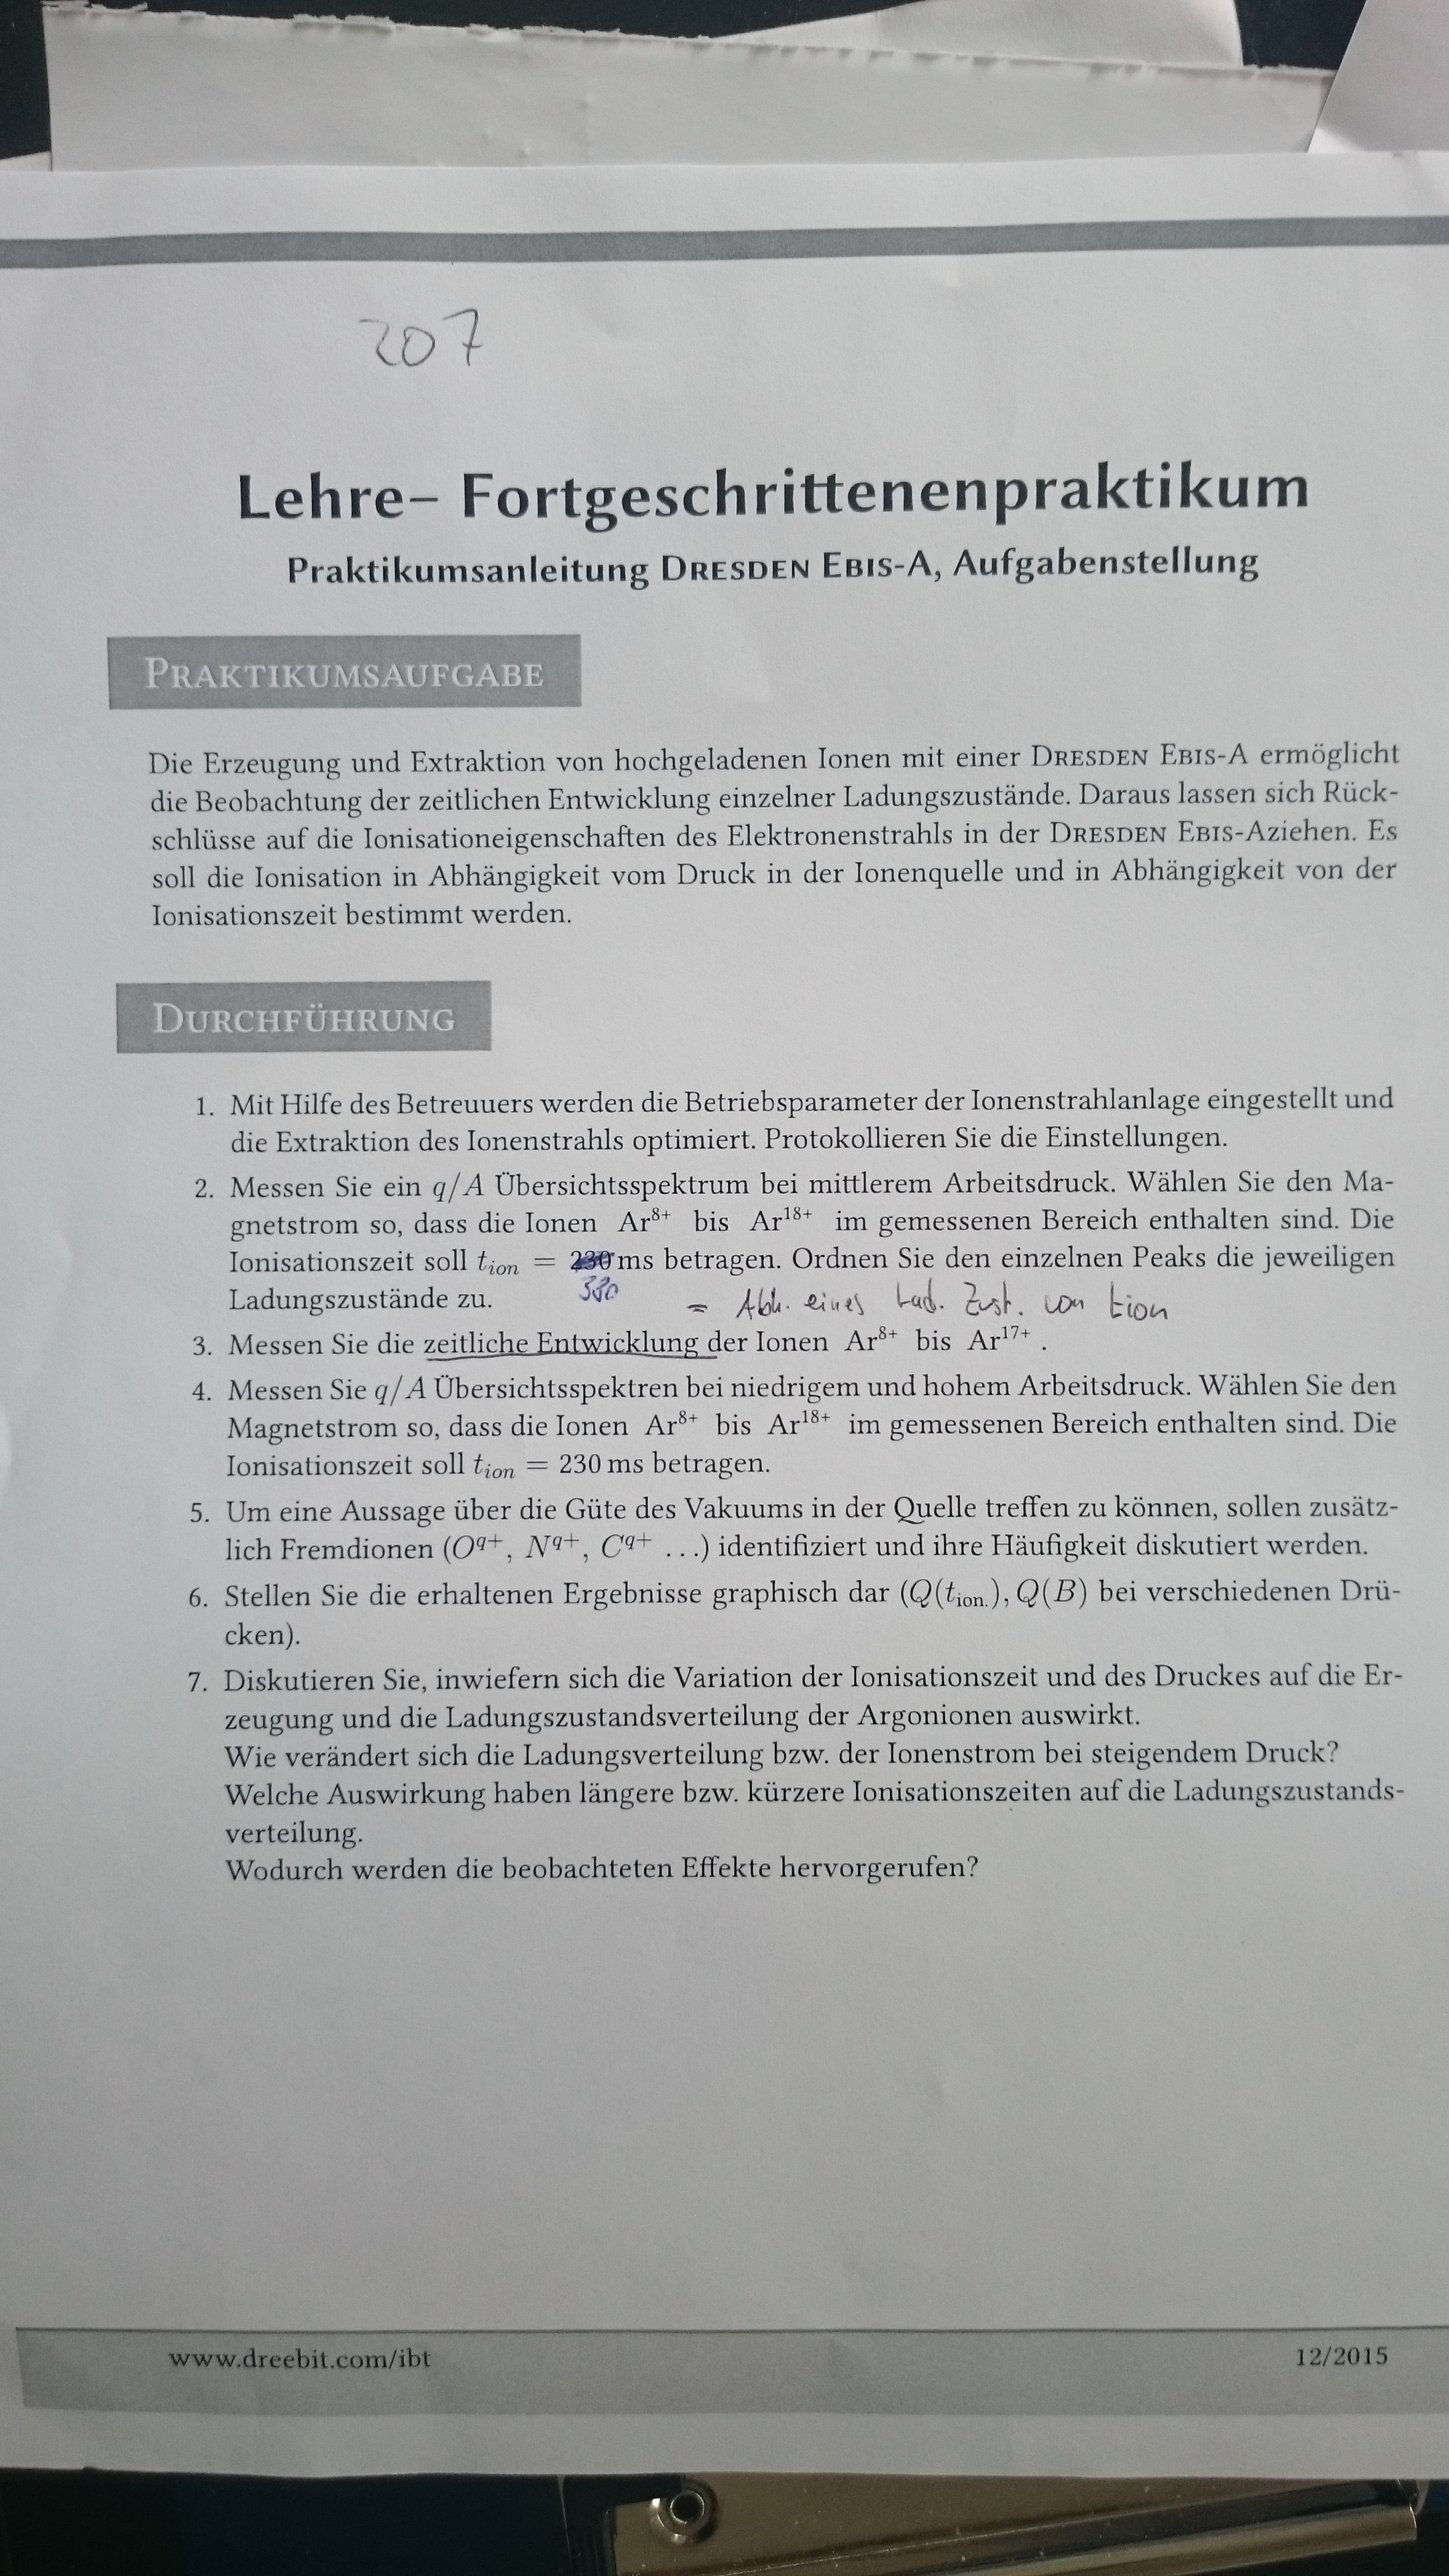
\includegraphics[scale=0.14]{../Mitschriften/DSC_0095.JPG}\\ \newpage
    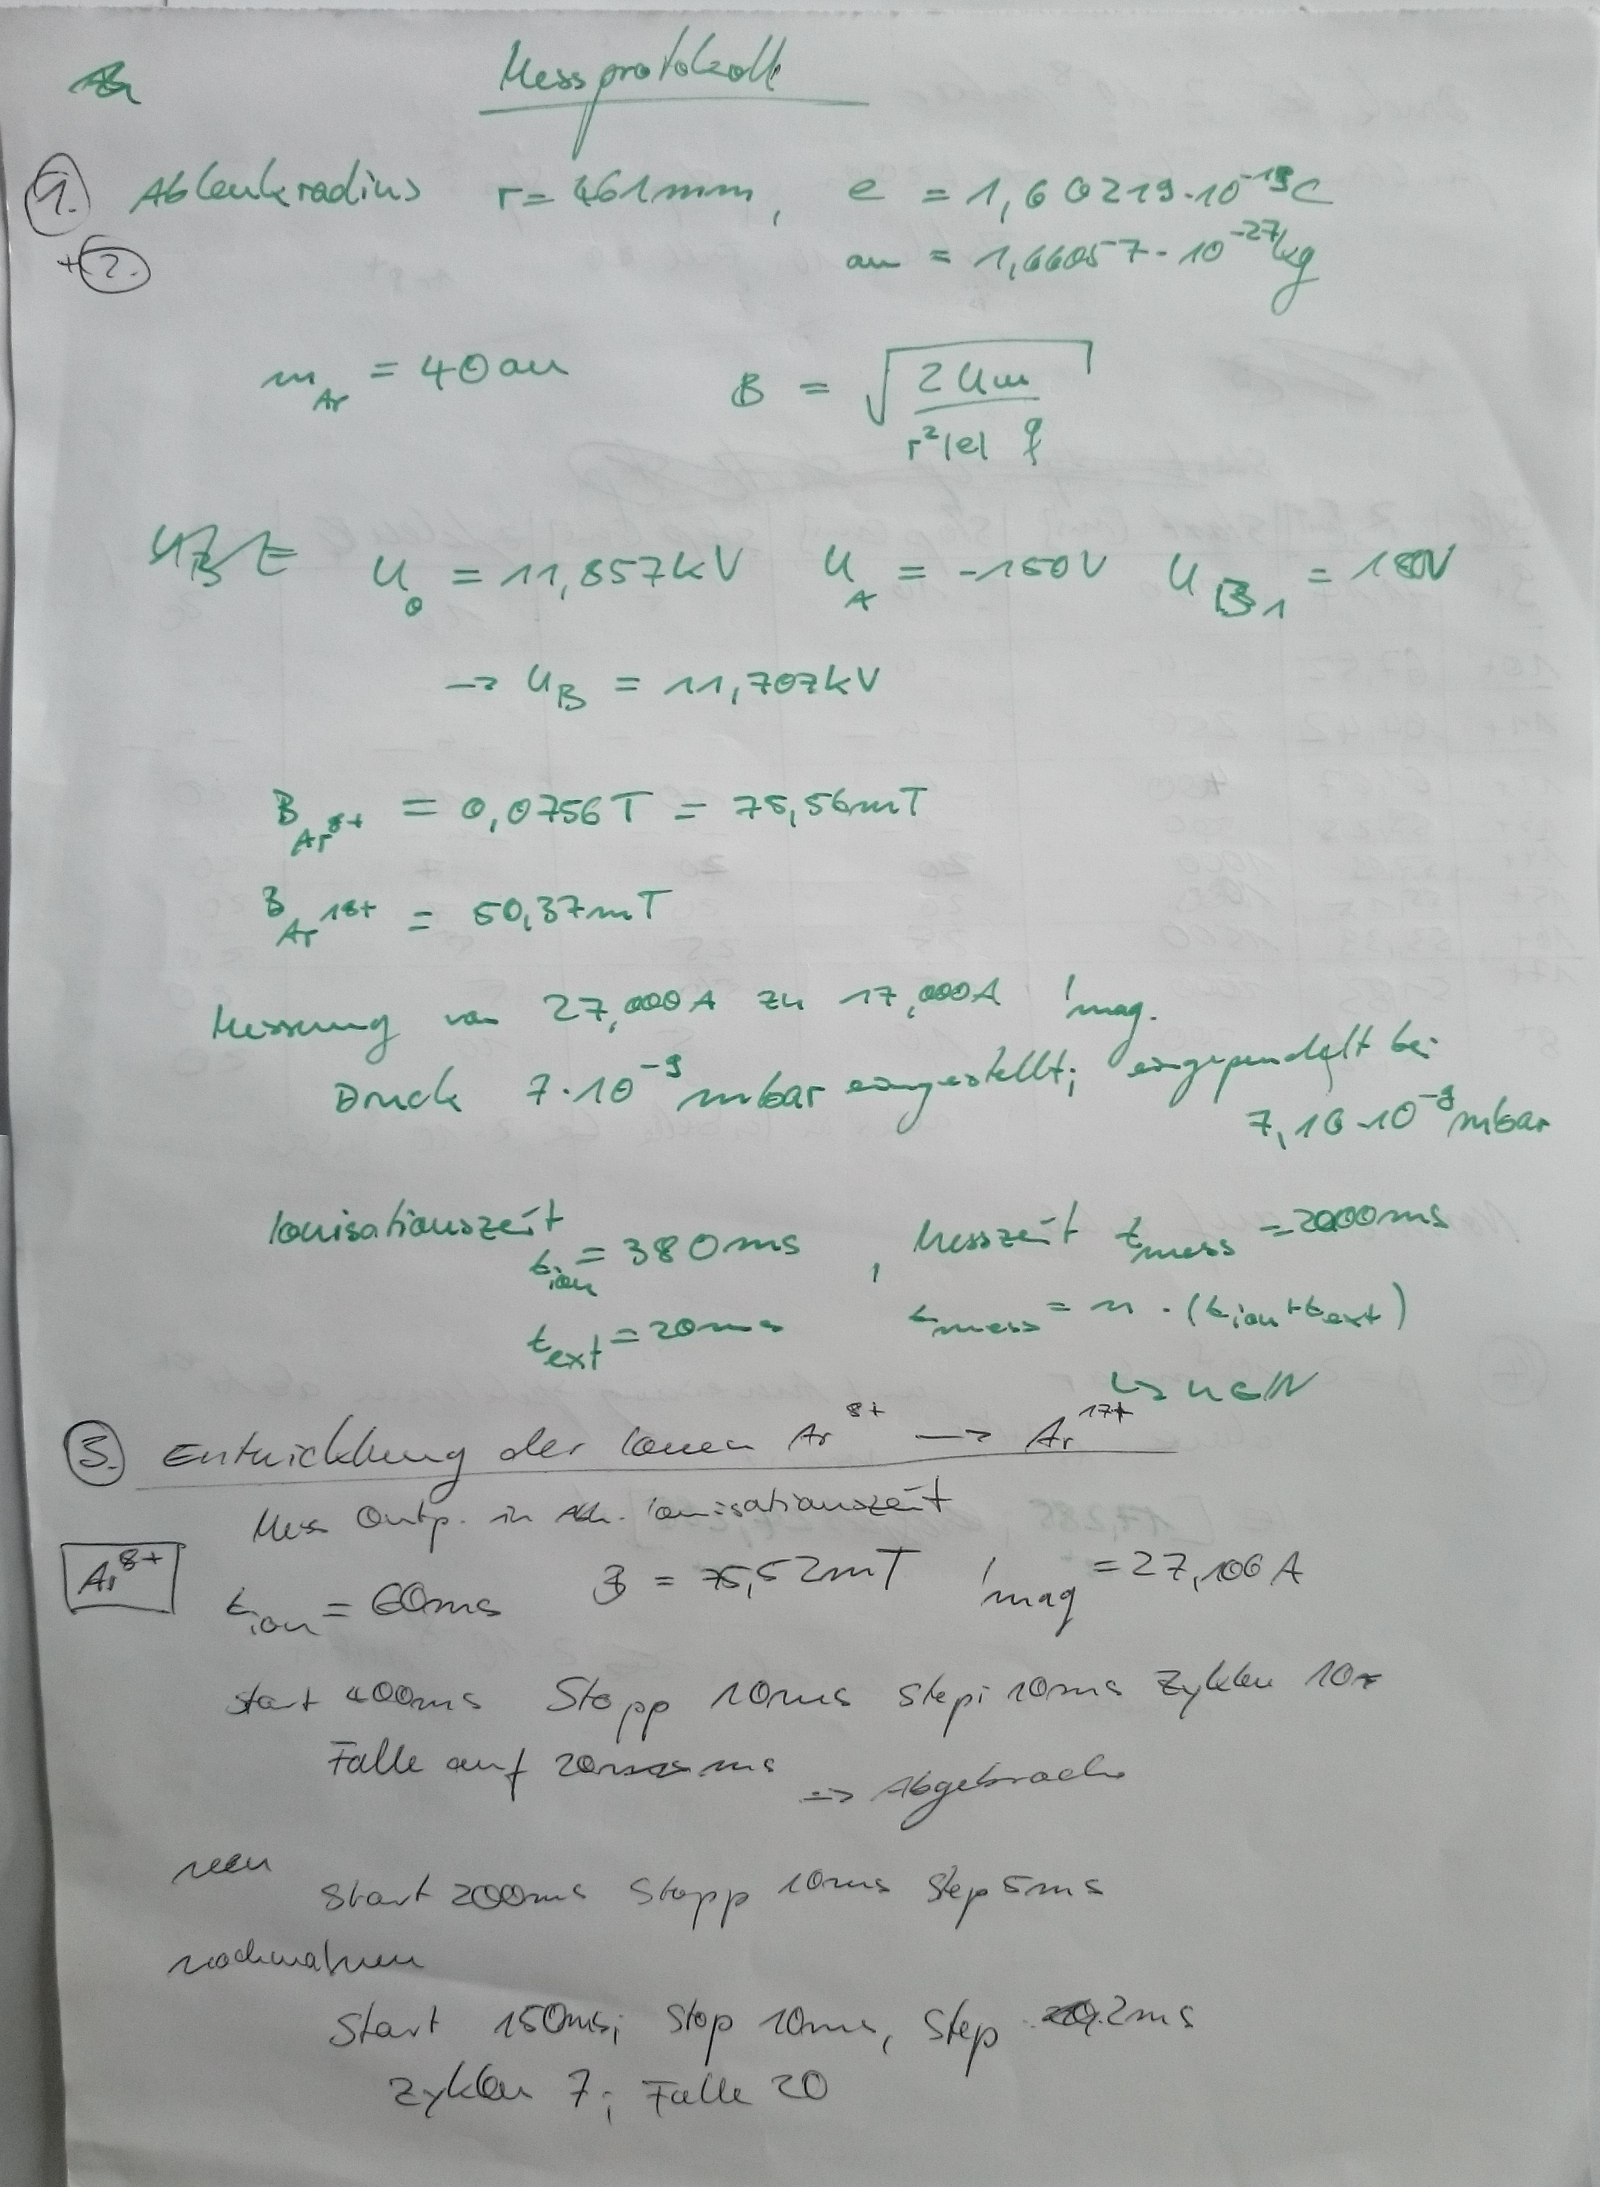
\includegraphics[scale=0.28]{../Mitschriften/DSC_0096.JPG}\\ \newpage
    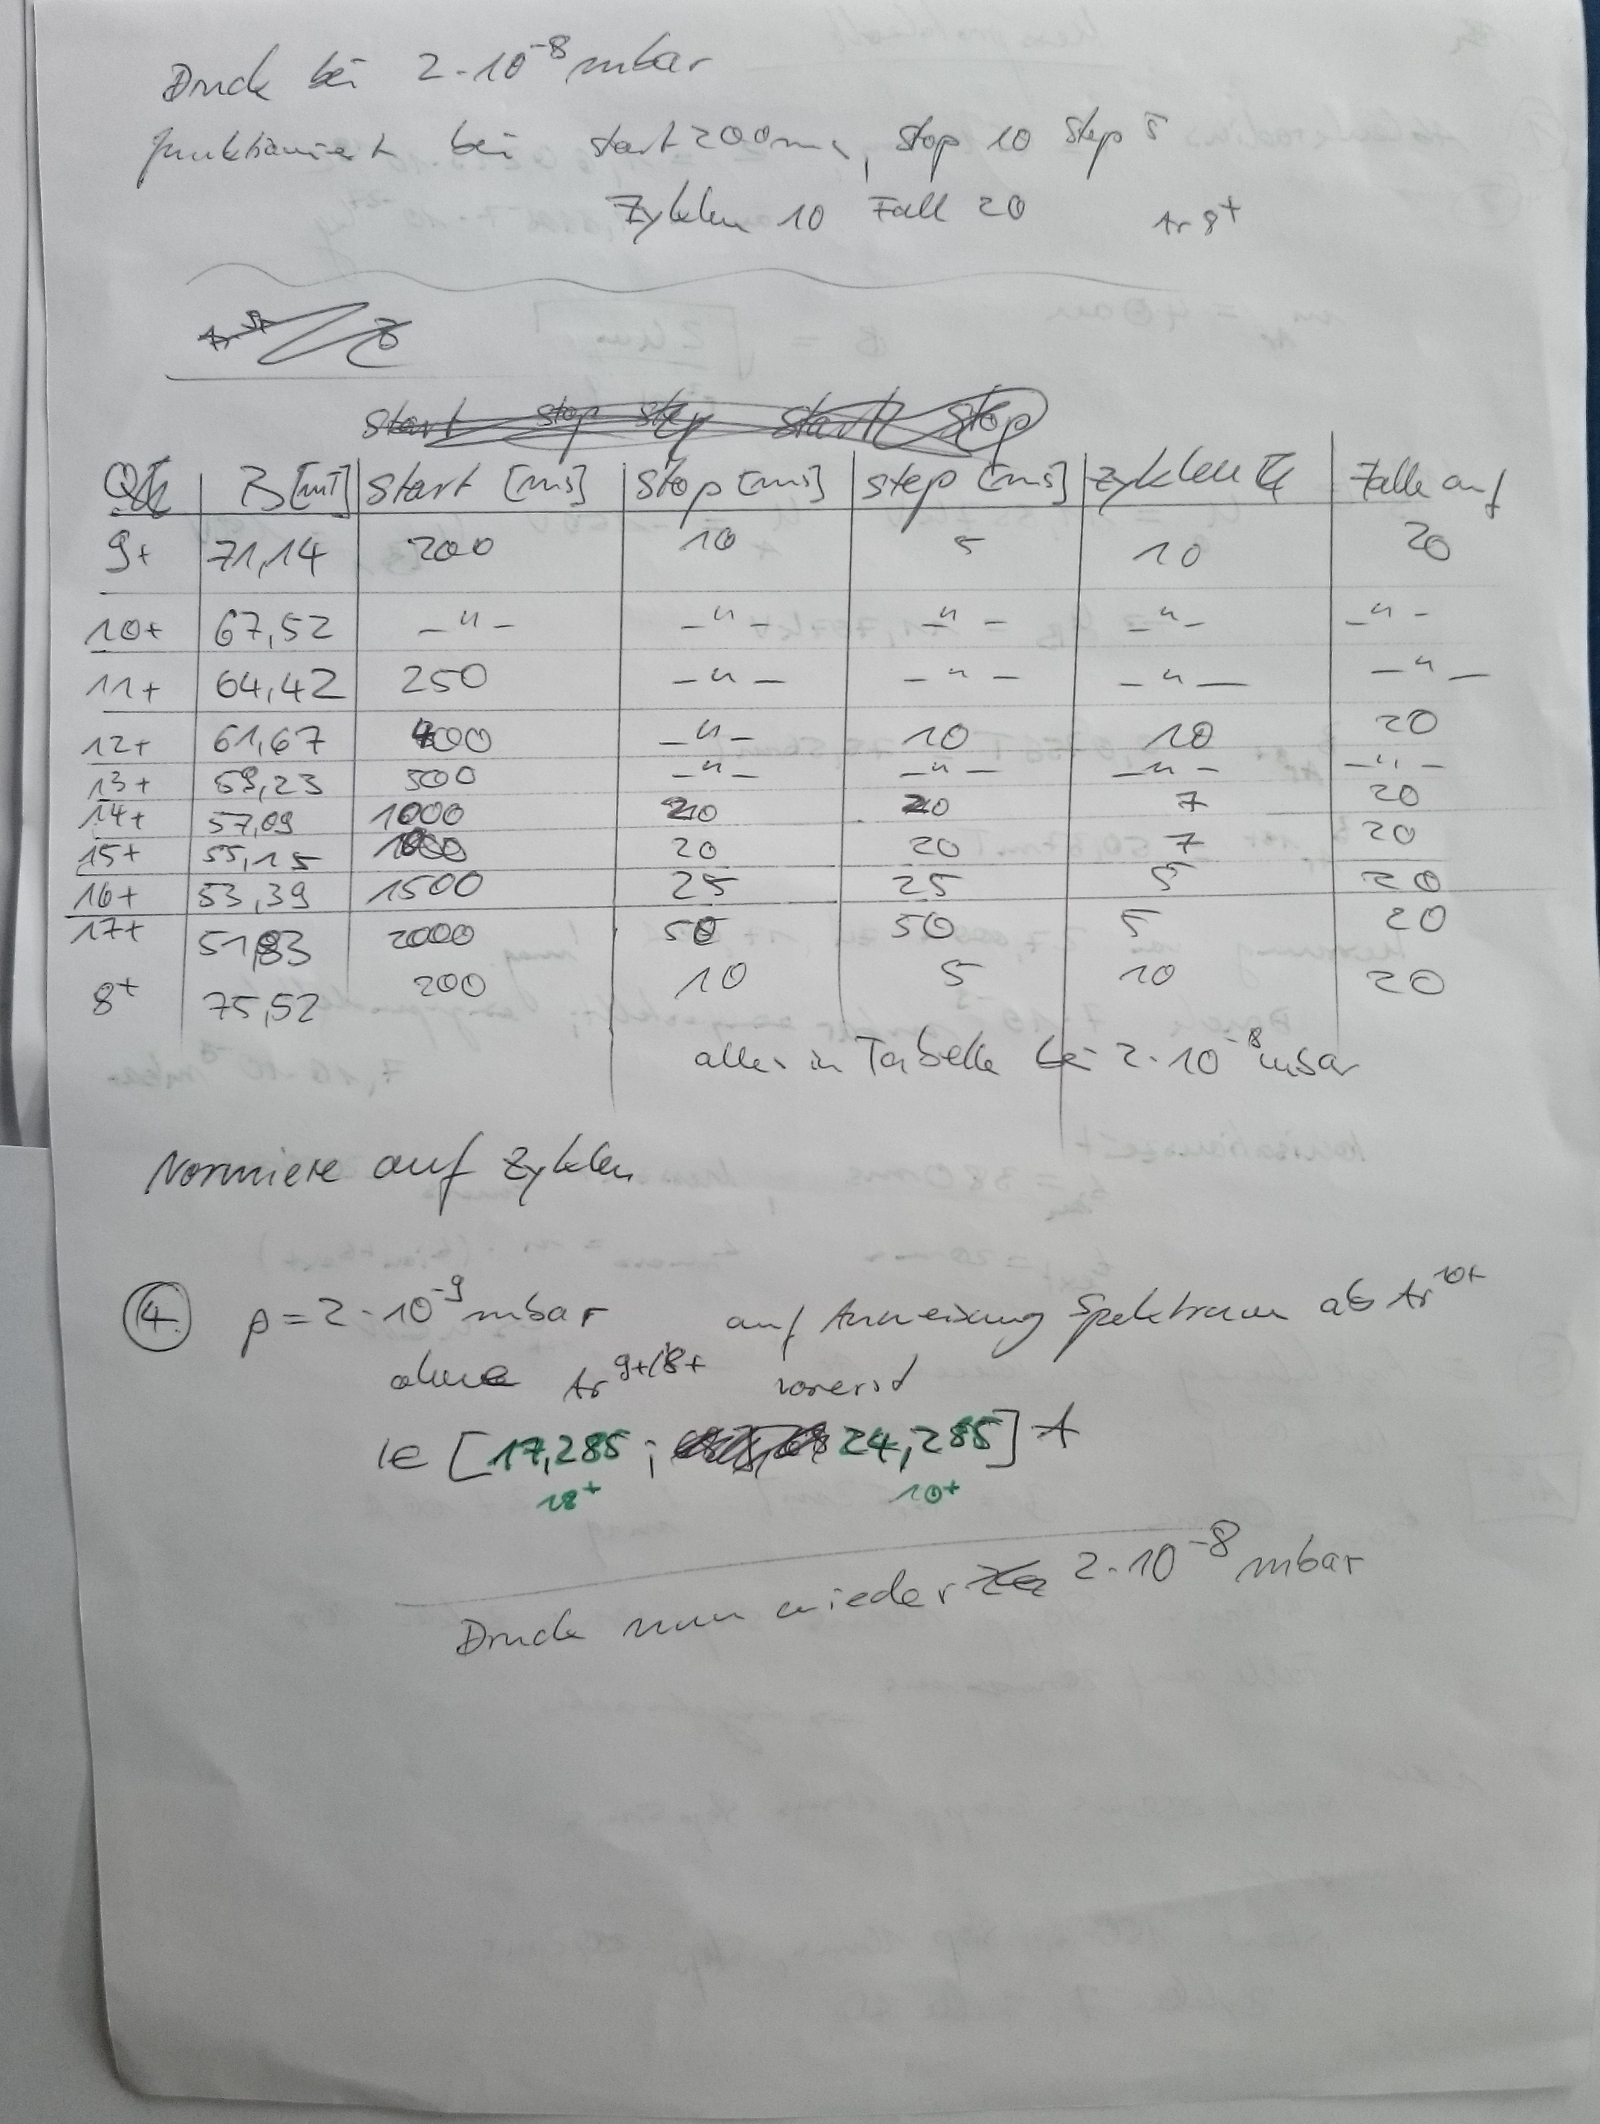
\includegraphics[scale=0.28]{../Mitschriften/DSC_0097.JPG}